\documentclass[a4paper,11pt]{article}
\usepackage{f420}
\DeclareMathOperator{\splay}{Splay}
\begin{document}

\section{Splay-деревья. Операция \texorpdfstring{\(\splay\)}{Splay}}

{\it Splay-дерево} представляет из себя самонастраивающуюся (self-adjusting) форму бинарного дерева поиска, выполняющую базовые операции над деревьями (такие как \(search, insert, delete\)) за амортизированное время \(O(\log{n})\).

Рассмотрим некоторое дерево и вершину \(x\) в нём. Введём операцию \(\splay(x)\), которая представляет из себя последовательность шагов zig, zig-zig и zig-zag (см.~рис.~\ref{fig:zigas}), причём после применения данной операции вершина \(x\) становится корнем дерева. Заметим, что шаг zig может быть лишь последним шагом и выполняться не более одного раза.

\begin{figure}[h] \centering
    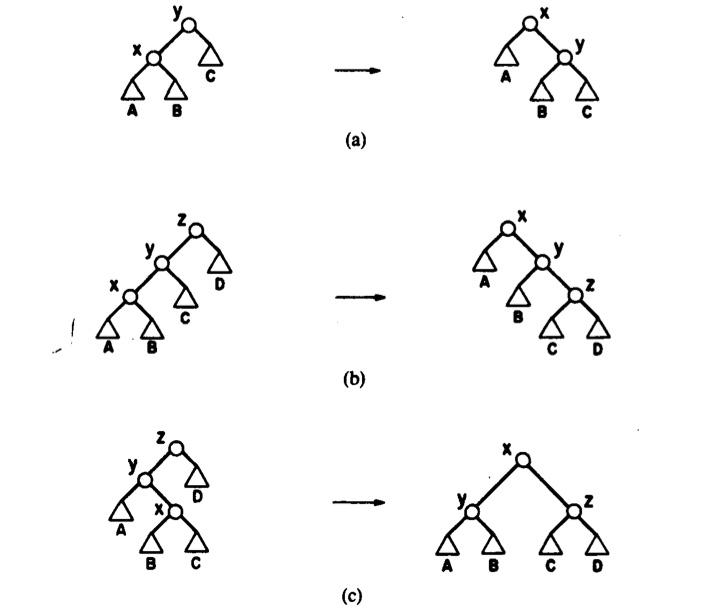
\includegraphics[scale=.5]{img/zigas.png}
    \caption{Шаг операции \(\splay(x)\). (a) zig: оканчивающий единичный поворот. (b) zig-zig: два единичных поворота. (c) zig-zag: двойной поворот.}
    \label{fig:zigas}
\end{figure}

\section{Амортизационный анализ}

Присвоим каждому элементу \(i\) вес \(w(i)\) -- произвольное положительное число; назовём размером \(s(x)\) вершины \(x\) сумму всех весов элементов в поддереве с корнем \(x\) (вершина \(x\) входит в это поддерево); назовём рангом \(r(x)\) вершины \(x\) величину \(\log{s(x)}\). Наконец, потенциалом \(\Phi(t)\) дерева \(t\) назовём сумму всех рангов всех вершин дерева \(t\).

Введём амортизированное время работы операции \(a = t + \Phi' -\Phi\), где \(t\) -- истинное время работы операции, \(\Phi'\) -- потенциал дерева после выполнения операции, а \(\Phi\) -- потенциал до операции. С таким определением мы можем вычислять общее время работы \(m\) операций, пользуясь следующей формулой:
\begin{align}\label{eq:1}
    \sum_{i=1}^m{t_i} = \sum_{i=1}^m{(a_i + \Phi_{i-1} - \Phi_{i})} = \sum_{i=1}^m{a_i} + \Phi_0 - \Phi_{m},
\end{align}
где \(t_i\) и \(a_i\) есть истинное и амортизированное время \(i\)-ой операции соответственно, \(\Phi_0\) -- начальный потенциал, \(\Phi_i\) -- потенциал после \(i\)-ой операции.


\begin{lemma}(Access lemma)
    Амортизированное время работы операции \(\splay(x)\) для дерева с корнем \(t\) не превосходит \(3(r(t) - r(x)) + 1 = O(\log{(s(t)/s(x))})\)
\end{lemma}

\begin{proof}
    Рассмотрим один шаг операции \(\splay{(x)}\) (т.е. или zig, или zig-zig, или zig-zag). Пусть \(s\) и \(s'\), \(r\) и \(r'\) -- размер и ранг до и после очередного шага соответственно. Утверждается, что амортизированное время шага zig не превосходит \(3(r'(x)-r(x)) + 1\), а для шагов zig-zig и zig-zag не превосходит \(3(r'(x)-r(x))\). Пусть вершина \(y\) является родителем вершины \(x\). Покажем заявленную оценку, например, для шага zip:
    \begin{align*}
        1 + r'(x) + r'(y) - r(x) - r(y) 
        & &\text{так как только }x \text{ и } y \text{ могут изменить ранг} \\
        \leq 1 + r'(x) - r(x) & &\text{так как } r(y) \geq r'(y) \\
        \leq 1 + 3(r'(x) - r(x))  & &\text{так как } r'(x) \geq r(x).
    \end{align*}
    Осталось заметить, что, просуммировав все оценки и сократив всё необходимое, получится оценка \(3(r'(x) - r(x)) + 1 = 3(r(t) - r(x)) + 1\), где \(r\) и \(r'\) -- ранги уже до и после всей операции \(\splay\) соответственно. 
    
\end{proof}

 

\begin{theorem}(Balance theorem)
    Рассмотрим splay-дерево на \(n\) вершинах, к которому выполняется \(m\) обращений к элементам. Тогда общее время работы есть \(O((m+n)\log{n} + m)\)
\end{theorem}

\begin{proof}
    Положим \(W = \sum_{i=1}^n{w(i)}\). Нетрудно заметить, что после последовательности обращений общая потеря в потенциале не превосходит \(\sum_{i=1}^n \log{(W/w(i))}\) в силу того, что размер вершины с элементом \(i\) не превосходит \(W\) и хотя бы \(w(i)\).
    
    Присвоим каждому элементу вес \(1/n\); отсюда имеем \(W = 1\). Значит амортизированное время запросов не превосходит \(3\log{n} + 1\) по предыдущей лемме; и при этом потеря в потенциале не превосходит \(n\log{n}\). Отсюда из \ref{eq:1} теорема верна.
\end{proof}

Заметим, что если выполняется достаточно много запросов к дереву (а именно в случае, когда \(m > n\)), то общее время работы есть \(O(m\log m)\). Другими словами, splay-дерево такое же эффективное, как и любая форма равномерно сбалансированного дерева.

\section{Операции, обновляющие splay-дерево}

\begin{itemize}
    \item \(access(i, t)\): выполняется поиск элемента \(i\), начиная с корня \(t\), спускаясь вниз по дереву. Если в процессе поиска достигается вершина \(x\), содержащая \(i\), то выполняется \(\splay(x)\) и возвращается указатель на \(x\). Если по итогу оказывается, что \(i\) нет в дереве, то выполняется \(\splay(x)\), где \(x\) -- последняя достигнутая в процессе поиска вершина.

    \item \(join(t_1, t_2)\): данная операция объединяет деревья \(t_1, t_2\) в одно дерево, предполагая, что любой элемент из дерева \(t_1\) строго меньше любого элемента из дерева \(t_2\). Для этого выполняется \(access\) наибольшого элемента элемента в дереве \(t_1\) (т.е. просто выполняется спуск в самый правый листочек). После \(access\)'а корнем дерева \(t_1\) является наибольший элемент этого дерева, т.е. корень не имеет правого ребёнка; соответсвенно можно правым ребёнком сделать корень дерева \(t_2\).

    \item \(split(i, t)\): данная операция строит деревья \(t_1, t_2\) так, что \(t_1\) содержит все элементы из \(t\), не превосходящие элемента \(i\), а \(t_2\) содержит все элементы из \(t\), строго большие элемента \(i\). Для этого выполняется \(access(i, t)\); после чего уничтожается одно из двух ребер, исходящих из корня, в зависимости от того, корень содержит элемент, больший или небольший чем \(i\).

    \begin{figure}[h] \centering
        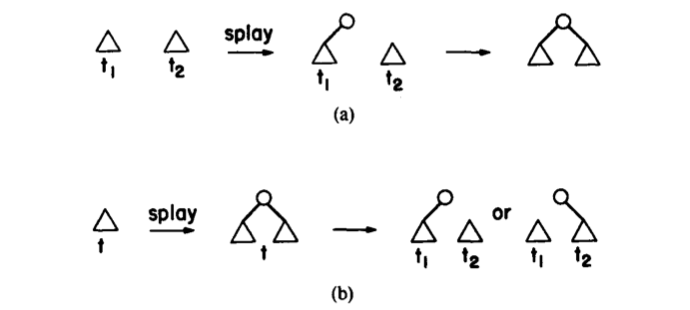
\includegraphics[scale=.5]{img/update1.png}
        \caption{Реализация \(join\) и \(split\). (a) \(join(t_1,t_2)\). (b) \(split(i, t)\).}
        \label{fig:update1}
    \end{figure}
    
    \item \(insert(i, t)\): выполняется \(split(i, t)\); после чего полученные деревья \(t_1, t_2\) делаем поддеревьями новой вершины, содержащей элемент \(i\) (операция \(insert\) выполняется при условии, что элемента \(i\) нет в дереве \(t\)).
    
    \item \(delete(i, t)\): выполняется \(access(i, t)\); после чего дерево \(t\) заменяется \(join\)'ом его левых и правых поддеревьев (операция \(delete\) выполняется при условии, что элемент \(i\) присутствует в дереве \(t\)).

    \begin{figure}[h] \centering
        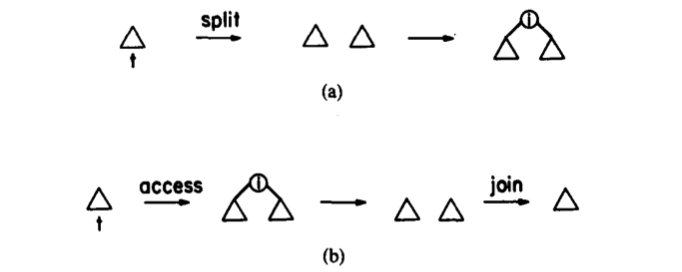
\includegraphics[scale=.5]{img/update2.png}
        \caption{Реализация \(insert\) и \(split\). (a) \(insert(i, t)\). (b) \(delete(i, t)\).}
        \label{fig:update2}
    \end{figure}
    

    
\end{itemize}



\end{document}
